\section{Network lifetime evaluation}
\label{PerformanceEvaluation}

This section describes the evaluation of the network lifetime extension algorithm.  We measure (a) the average number of switches to form the improved tree and (b) the impact of swapping on the network lifetime.  As mentioned in section \ref{OptimalTree} we define the network lifetime as the time until first node failure, that is the smallest value of $l_i$ from (\ref{optimalEq}).  Because lifetimes must be evaluated over extremely long periods with large numbers of nodes, simulation is used instead of emulation.

\subsection{Simulation Setup}

The improved tree algorithm from section \ref{OptimalTree} is simulated in the C programming language. The number of sensors considered is varied between 10 to 500 and each node is randomly assigned an initial energy between 50\% to 100\%. The link conditions are also randomly assigned the value between 1 to 10 indicating the ETX (1 being a clear channel with no retransmission and 10 meaning ten retransmissions on average). In this setup, the channels are fixed, assuming that the current channels that the nodes are listening and transmitting on, are the best selected channels from the previous MCRP processes. RPL builds the initial tree based on the ETX value which is then further improved by MCRP. In order to avoid all the nodes from directly connecting to the LPBR, each node could route to a minimum of $1/10$ and $1/30$ of the total number of nodes.
This allows the node to have alternative parents (thus paths) for the swapping processes and hops to reach the LPBR. The node is not necessarily connected to all $1/10$ and $1/30$ nodes. The paths between the nodes are selected based on the RPL and MCRP processes. These values are selected in the case where (a) the nodes are closely together ($1/10$), and (b) the nodes are spread out with minimum connections to the other nodes available ($1/30$). 

\subsection{Simulation Results}
\subsubsection{Average Number of Switches}

\begin{figure}
\centering
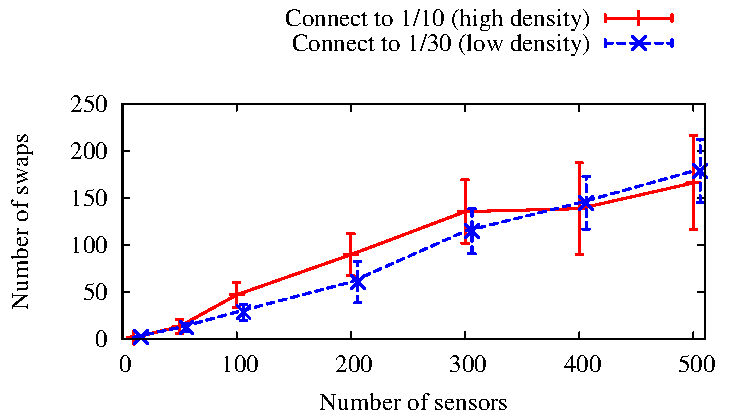
\includegraphics[width=0.45\textwidth]{figures/swaps.pdf}
\caption{Simulation: Average number of swaps}
\label{fig:aveSwaps}
\end{figure}

Figure \ref{fig:aveSwaps} shows the standard deviation and average number of swaps using MCRP improved tree algorithm. 
It can be observed that there are more swaps on average when there are more sensors in the network in both connection cases. However, nodes that could route to $1/10$ of the total sensors showed slightly higher number of swaps than in the $1/30$ connection. The reason for this is because in $1/10$ connection, it has more neighbours, hence many potential parents to select. 

In a smaller network, the sensors are limited by the number of potential parents. This prevents the nodes from swapping as the potential parents might not have any improvement. This can be seen from the number of swaps in a 50 sensors network where the average number of swaps is less than 10. This is because each node has 5 (in $1/10$) and 2 (in $1/30$) potential parents to select from unlike in the 500 sensors network which each has 50 and 17 potential parents. However, as there are more sensors, it takes longer to find the best parents as the swaps will consider all nodes that are within the range.

This experiment does not reflect the condition in the real world where the sensors could be scattered with more or less available range to the other nodes depending on the application; which means more nodes can directly be connected to the LPBR without hops in between. This however, represents a reasonable connection between the nodes to allow swapping and alternative nodes if the current forwarding nodes values are at a minimum for the experiment.


\subsubsection{Impact On The Network Lifetime}

\begin{figure}
\centering              
\subfigure[Connect to 1/10 of total sensors]{\label{fig:1-10}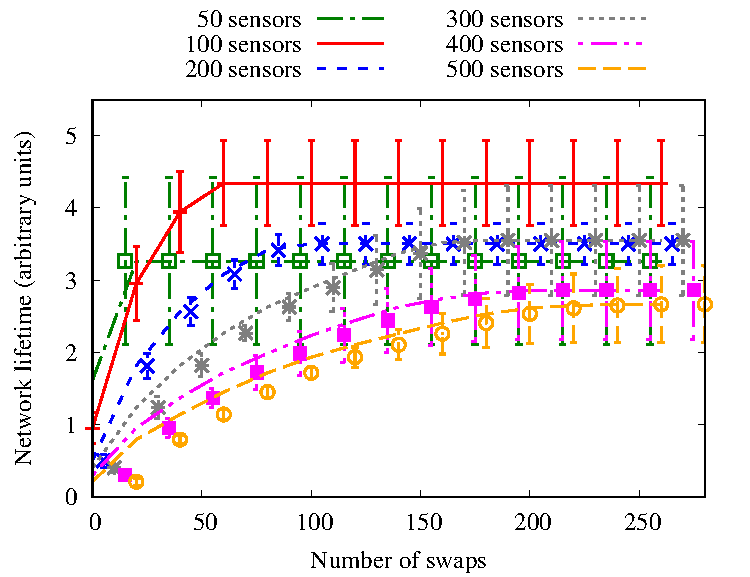
\includegraphics[width=0.45\textwidth]{figures/lifetime1.pdf}}
\subfigure[Connect to 1/30 of total sensors]{\label{fig:1-30}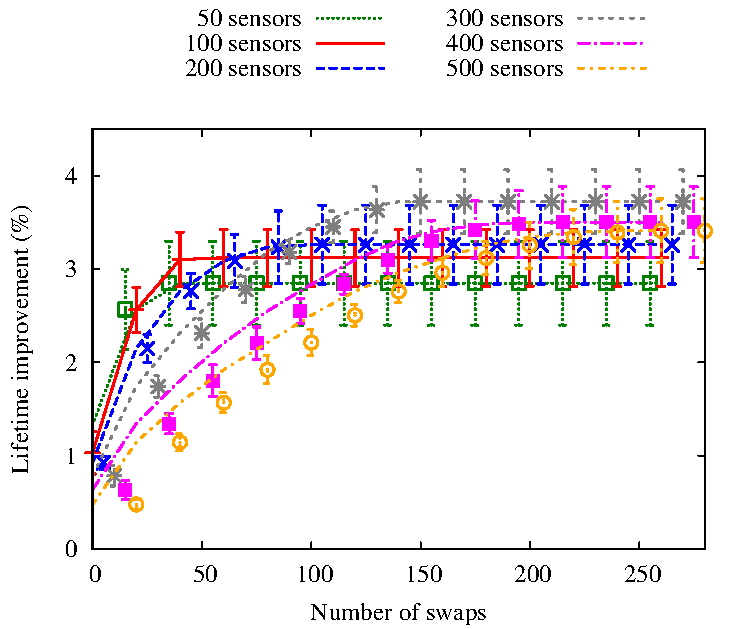
\includegraphics[width=0.45\textwidth]{figures/lifetime3.pdf}}
\caption{Simulation: Comparison of the number of swaps and lifetime in different network scale}
\label{fig:maxmin}
\end{figure}

Figure \ref{fig:maxmin} shows the improvement in the node thus network lifetime by maximising the minimum and the number of swaps required in 10 runs in 6 networks with 50, 100, 200, 300, 400 and 500 sensors with different degree of connection. 
The standard deviation on the x axis is slightly shifted to prevent the error bars from overlapping.
It is observed that the node lifetime decreases with an increase in the number of sensors in the network. The reason for this is in a larger network, there are a higher number of descendants and each connection has its own path values. By taking into account these variables, the number of nodes affect the whole network lifetime. While a higher number of nodes allow more alternative routes, it also consumes more energy as there are more connected nodes. Smaller network however, has limited number of possible swaps which does not improve the network lifetime.

Figure \ref{fig:1-10} shows the number of swaps and the lifetime when the nodes are connected to $1/10$ of the total nodes in the network. 
In the 50 nodes network, the number of swaps is less than 10 before it reaches the maximum lifetime for the whole network. 
As the number of sensors in the network increase, it takes more swaps before the tree is improved. 
In the 200 nodes network, the number of swaps is around 100 swaps and the lifetime is improved by a factor of 7, an increase from 0.5 to 3.5. In 500 nodes network, it takes more swaps, around 200 swaps for the lifetime is improved by a factor of 9, an increase from 0.3 to 2.7.

Figure \ref{fig:1-30} shows similar improvement in the $1/30$ connection case. However, it can be seen that the maximum lifetime values in the figure for 100 sensors network is slightly less than in Figure \ref{fig:1-10}. This is because the networks have lesser potential parents and paths to select from. The tree is limited by the number of connections. The other large networks have similar maximum lifetime values in both figures.

\begin{figure}
\centering
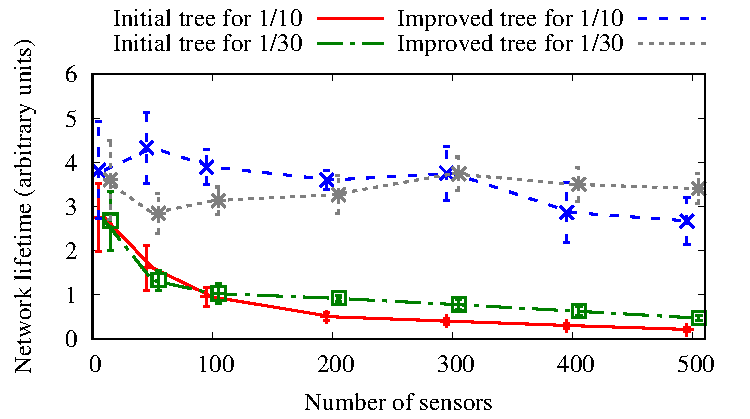
\includegraphics[width=0.45\textwidth]{figures/maxmin.pdf}
\caption{Simulation: Lifetime of MCRP improved tree}
\label{fig:nodes-maxmin}
\end{figure}

Figure \ref{fig:nodes-maxmin} shows the comparison between the initial and improved tree in both cases. MCRP swapping prolongs the network lifetime which shows an increase from the initial lifetime. Smaller networks have high initial lifetime values compared to larger networks.  This is because in large networks there are always a few nodes that have to carry a great amount of traffic.  However, larger networks have better lifetime improvement than the slight improvement in smaller networks.

In the initial trees, it can be seen that when there are more sensors in the network, the lifetime values are decreasing. This shows the importance of finding the improved tree as the results showed that the lifetime can be improved by a factor of 9 in the 500 nodes network.
%four times. 
The increase enables the network to remain functional slightly longer than initially. 

